%!TEX program = pdflatex
\documentclass[10pt]{article}
\usepackage[pdftex]{graphicx, color}
\usepackage{listings}
\usepackage{forest}
\usepackage{tikz}
\usetikzlibrary{automata,positioning}

\headheight 8pt \headsep 20pt \footskip 30pt
\textheight 9in \textwidth 6.5in
\oddsidemargin 0in \evensidemargin 0in
\topmargin -.35in

\lstset{basicstyle=\small\ttfamily,breaklines=true}
\newcommand {\pts}[1]{{\bf #1 pts}}

\begin{document}
\begin{center}
\Large CS131 Compilers: Writing Assignment 2\\Due Saturday, April 10, 2021 at 23:59pm
\end{center}

\begin{center}
%% Change this:
\LARGE Name - Number
\end{center}

This assignment asks you to prepare written answers to questions on
context-free grammars and parsing. Each of the questions has a short answer. You
may discuss this assignment with other students and work on the problems
together. However, your write-up should be your own individual work.
and you should indicate in your submission who you worked with, if applicable.
Written assignments are turned in at the start of lecture.
You should use the Latex template provided at the course web site to write your solution.

\begin{center}
%% Change this:
I worked with: ()()
\end{center}

\begin{enumerate}
  \item  \pts{$2*2+8 = 10$} Give context-free grammar (CFG) for each of the following languages, for the last part, you don't need to draw the tree but the semantic alongside with the production rule:
  \begin{enumerate}
           \item The set of all finite strings over the alphabet $\{0,1\}$ with an unequal number of 0's and 1's.
          \[
          $$  
          S $\to$ $A0A$ $|$ $A1A $\\
          A $\to$ $AA$ \\
          $A$ $\to$ $0A1$ $|$ $1A0$\\
          A $\to$ $\epsilon$\\
          $$
          \]
            \item The set $L_3=L_1\cap L_2$, where $L_1$ and $L_2$ are defined below.
            Let $L_1$ be the finite strings consisting of all non-empty \emph{palindromes} over the alphabet $\{a,b\}$. 
            
            For example, $abba,~aabbbaa\in L_1$, but $abb\not\in L_1$.
            Let $L_2$ be the language over  $\{a,b\}$ representing the language of the regular expression $b(a+b)^\ast$.
             \[
             $$
                S $\to$ bBb \\
                B $\to$ aBa $|$ bBb $|$ $\epsilon$
             $$
             \]
           \item The set of all finite strings over the alphabet $\{0,1\}$ that generate all the binary number including digits (e.g. 110.0110). 
            \[
            %% Your answer here
            \]
            \begin{enumerate}
              \item Write the syntax-directed translation scheme (SDT) with S-attributed definition.
              \[
                $$
                \begin{center}
                  \begin{tabular}{ l | c  }
                    \hline
                    S $\to$ L &  S.v = L.v \\ 
                    S $\to$ $L_1.L_2$&  S.v = $L_1$.v + $L_2$.v /  $2^{L_1.len}$\\ 
                    L $\to$  $L_1B$ & L.v = $L_1.v$*2+B.v, L.len++\\
                    L $\to$ B & L.v = B.v, L.len=1\\
                    B $\to$ 0 $\mid$ 1 & B.v = I \\
                    \hline
                  \end{tabular}
                \end{center}
                $$
                \]
              \item Write the syntax-directed translation scheme (SDT) with L-attributed definition.
              \[
                $$
                \begin{center}
                  \begin{tabular}{ l | c  }
                    \hline
                    S $\to$ L &  S.v = L.v \\ 
                    S $\to$ $L_1.L_2$&  S.v = $L_1$.v + $L_2$.v /  $2^{L_1.len}$\\ 
                    L $\to$  $L_1B$ & L.v = $L_1.v$*2+B.v, L.len++\\
                    L $\to$ B & L.v = B.v, L.len=1\\
                    B $\to$ 0 $\mid$ 1 & B.v = I \\
                    \hline
                  \end{tabular}
                \end{center}
                $$
                \]
              \item Using the CFG you wrote, provide a derivation for the following input string: 10.1011
              \\
              \begin{forest}
                [, phantom, s sep = 1cm
                 [{$S.v = 2 + 11/ 2^{2}$}[{$L.v=2, L.len=2$}[{$L.v = 1,L.len=1$}[1]][{0}]][.][{$L.v=11,L.len=4$}[{$L.v=5,L.len=3$}[{$L.v=2,L.len=2$}[{$L.v=1,L.len=1$}[1]][{0}]][1]][{1}]]]
                ]
                \end{forest}
            \end{enumerate}
  \end{enumerate}
  %


   
\item \pts{$3\times 3= 9$} Consider the following CFG.
\[\begin{array}{cll}
S & \rightarrow & G \\
G & \rightarrow & P \mid P G \\
P & \rightarrow & \textbf{id}: R\\
R & \rightarrow & \epsilon \mid \textbf{id}R 
\end{array}\]

\begin{enumerate}
\item What is the language generated by this grammar?
       \[
       $$
        The language generated by this grammar is { $[[\textbf{id}:][\textbf{id}]*]+ $ }
       $$  
       \]
\item Is the grammar as given ambiguous? If yes, give an example of an expression
with two parse trees under this grammar. If not, explain why that is the case.
            \[
            $$
              The grammar is unambiguous. Because Unambiguous Grammar has exactly one set of handles for a Right-most Derivation, and \textbf{id}:R and \textbf{id}R are exactly two separate rules, which contributes to one parser tree.
            $$
            \]
\item Transform the CFG given above by eliminating ambiguity and
left recursion, if needed.
            \[
            $$
              There's no need since it's unambiguous.
            $$
            \]
\end{enumerate}

\newpage
\item \pts{$3\times 3= 9$} Consider the following CFG.
\[\begin{array}{cll}
S & \rightarrow & (  X \\
S & \rightarrow & E] \\
S & \rightarrow & F) \\
X & \rightarrow & E) \\
X & \rightarrow & F] \\
E & \rightarrow & A \\
F & \rightarrow & A \\
A & \rightarrow & \epsilon
\end{array}\]

\begin{enumerate}
  \item Compute the Nullable, First and Follow sets for the grammar.
             \[
            $$
            Nullable(S) = True  \\
            Nullable(X) = True  \\
            Nullable(E) = True  \\
            Nullable(F) = True  \\
            Nullable(A) = True  \\
            \\
            First(S) = $\{ (,\epsilon \}$\\
            First(X) = $\{ \epsilon, ), ] \}$\\
            First(F) = $\{ \epsilon \}$\\
            First(E) = $\{ \epsilon , ), ]\}$\\
            First(A) = $\{ \epsilon , ), ]\}$\\

            Follow(S) = $\{ \$\}$\\
            Follow(E) = $\{ ] ,)\}$\\
            Follow(F) = $\{ ) ,] \}$\\
            Follow(X) = $\{  \$ \}$\\
            Follow(A) = $\{ ) ,] \}$
            $$
            \]
  \item Give the LL(1) parsing table for the grammar.
  \begin{center}
    
 
    \[
    $$ 
   
    \begin{table}[h!]
      \begin{tabular}{|c|c|c|c|c|}
      \hline
      Non-terminal           &                        &                        & INPUT SYMBOL             &                                                                   \\ \hline
      \multicolumn{1}{|l|}{} & \multicolumn{1}{l|}{(} & \multicolumn{1}{l|}{)} & \multicolumn{1}{l|}{{]}} & \multicolumn{1}{l|}{\$}                                           \\ \hline
      S                      & S $\to$ X              &   S $\to$ E]        S $\to$ F)               &          S $\to$ E]        S $\to$ F)                   & \begin{tabular}[c]{@{}c@{}}S $\to$ E{]}\\ S $\to$ F)\end{tabular} \\ \hline
      X                      &                &                 X   $\to$  E)         &      X $\to$ F]                      & X $\to$ E)X $\to$ F{]}                                            \\ \hline
      E                      &                        & E $\to$ A              & E $\to$ A                &                                                                   \\ \hline
      F                      &                        & F $\to$ A              & F $\to$ A                &                                                                   \\ \hline
      A                      &                        & A $\to$ $\epsilon$     & A $\to$ $\epsilon$       &                                                                   \\ \hline
      \end{tabular}
      \end{table}
    $$
    \]
  \end{center}
  \item Is this grammar LALR(1)? and Why.
    \[
    $$
    No. There are conflicts in $E \to A$ and $F \to A$.
    $$  
    \]
\end{enumerate}

\item \pts{$8$}  Using the context-free grammar for Cool given in Section 11 of the Cool
manual, draw a parse tree for the following expression.
  \begin{lstlisting}
    while not (x <-z <- 0) loop
      y <- z + 2 * x + 1
    pool
  \end{lstlisting}
Note that the context-free grammar by itself is ambiguous, so you will
need to use the precedence and associativity rules in Section 11.1 to
get the correct tree.
         
\begin{forest}
  [, phantom, s sep = 1cm
    [expr
    [while] 
    [expr[not] [expr[[(][expr[ID[x]] [ \lstinline{<-} ] [expr[ID[z]][\lstinline{<-}][expr[integer[0]]]]][)]]]] 
    [loop]
    [expr[ID[y]][\lstinline{<-}][expr
    [expr[expr[ID[z]]][+][expr[expr[integer[2]]][*][expr[ID[x]]]]][+][expr[integer[1]]]
    ]]
    [pool]
    ]
  ]
  \end{forest}
  
         

\newpage
\item \pts{$4\times 4 =16$} Consider the following grammar describing a certain sort of nested lists:
\[\begin{array}{cll}
S & \rightarrow & T;S \mid \epsilon \\
T & \rightarrow & U\star T \mid U \\
U & \rightarrow & x\mid y\mid [S]
\end{array}\]
$S$, $T$, and $U$ are nonterminals, while others are terminals.
\begin{enumerate}
  \item Left-factor this grammar.
               \[
            $$
            S $\to$ T;S $|$ $\epsilon$ \\
            T $\to$ UT'\\
            T' $\to$  $\star T$ $|$ $\epsilon$ \\
            $U  \rightarrow  x\mid y\mid [S]$
            $$
            \]
  \item Give the First and Follow sets for each nonterminal in the grammar obtained in part (a).
               \[
            $$
            First(S) = $\{ x,y,[ , \epsilon \}$ \\
            First(T) = $\{ x,y,[   \}$ \\
            First(U) = $\{ x,y,[ \}$ \\
            First(T') = $\{ \star, \epsilon \}$ \\
            Follow(S) = $\{ ], \$ \}$ \\
            Follow(T) = $\{ ; \}$ \\
            Follow(U) = $\{ \star,; \}$ \\
            Follow(T') = $\{; \}$ \\
            $$
            \]
  \item Using this information, construct an LL(1) parsing table for the grammar obtained in part (a).
            \begin{center}
              \begin{table}[h!]
                \begin{tabular}{|l|l|l|l|l|l|l|l|}
                \hline
                Non-terminal &   & Input symbol &   &   &     &     &    \\ \hline
                             & ; & $\star$      & x & y & {[} & {]} & \$ \\ \hline
                S            &   &              &S $\to$ T;S   & S $\to$ T;S & S $\to$ T;S    & S $\to$  $\epsilon$    &   S $\to$  $\epsilon$ \\ \hline
                T            &   &              &  T $\to$ UT'  &  T $\to$ UT'  &   T $\to$ UT'   &     &    \\ \hline
                T'           &             T' $\to$   $\epsilon$  &             T' $\to$  $\star T$     &   &   &     &     &    \\ \hline
                U            &   &              & $U  \rightarrow  x$   & $U  \rightarrow   y$   &   $U  \rightarrow   [S]$   &     &    \\ \hline
                \end{tabular}
                \end{table}
            \end{center}
  \item Suppose we generated an LL(1) parser for the grammar using the table you constructed. What would go wrong if it tried to parse the following input string?
  \[[x;y]\star [;\]
               \[
            $$
                There's no rule accepting ; after [
            $$
            \]
\end{enumerate}

\newpage
\item \pts{$3\times 2+5\times 2 =16$} Consider the following CFG, which has the set of terminals
$T = \{ \textbf{a}, \textbf{b} , \textbf{c} \}$.
\[\begin{array}{cll}
X & \rightarrow & \textbf{c} \mid \textbf{a} X \textbf{b} X |  \textbf{a} X
\end{array}\]

\begin{enumerate}

\item Construct a DFA for viable prefixes of this grammar using LR(0)
items.

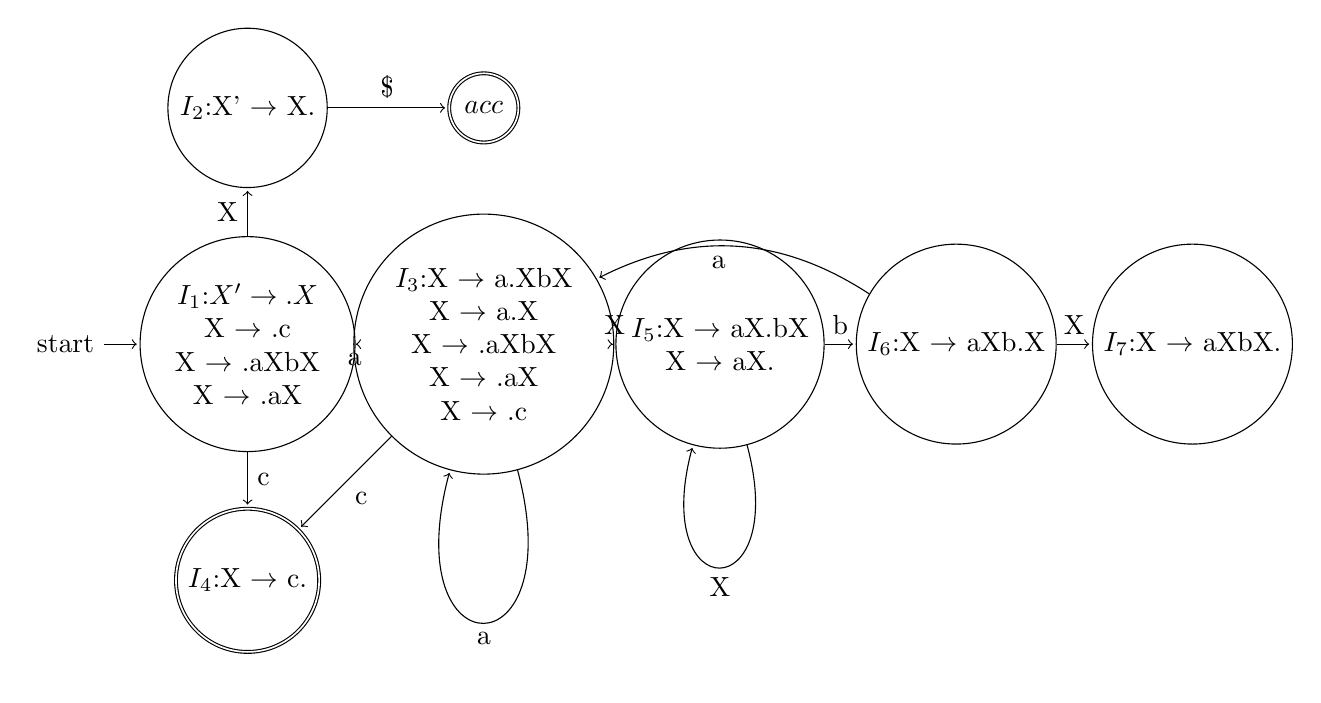
\begin{tikzpicture}[shorten >=1pt,node distance=3cm,on grid,auto, align=center]
    \node[state, initial] (1) {$I_1$:$X' \to .X$ \\X $\to$ .c\\X $\to$ .aXbX \\ X $\to$ .aX};
    \node[state ] (2) [above= of 1]  {$I_2$:X' $\to$ X.};
    \node [state, accepting] (8) [right = of 2] {$acc$};
    \node [state] (3) [right = of 1] {$I_3$:X $\to$ a.XbX \\ X $\to$ a.X \\ X $\to$ .aXbX \\ X $\to$ .aX\\X $\to$ .c};
    \node[state, accepting] (4) [below = of 1]{$I_4$:X $\to$ c.};
    \node [state] (5) [right = of 3] {$I_5$:X $\to$ aX.bX \\ X $\to$ aX. } ;
    \node [state] (6) [right = of 5] {$I_6$:X $\to$ aXb.X} ;
    \node [state] (7) [right = of 6] {$I_7$:X $\to$ aXbX.};
    % \node [state, accepting] (8) [right = of 7] {$8$};
    \path [ ->]
    % (1) edge [loop below] node {$c$} (1)
    % (1) edge  node {$a$} (2)
    % (2) edge [loop below] node {$a,c$} (2)
    % (2) edge node {$b$} (3)
    % (3) edge [loop below] node {$a,b,c$} (3)
    % (1) edge node {$b$} (e)
    (1) edge node {X} (2)
    (2) edge node {\$} (8)
    (1) edge node {c} (4)
    (3) edge node {c} (4)
    (1) edge node {a} (3)
    (3) edge [loop below] node {a} (3)
    (5) edge [loop below] node {X} (5)
    (3) edge node {X} (5)
    (5) edge node {b} (6)
    (6) edge [bend right] node {a} (3)
    (6) edge node {X} (7)
    ;
\end{tikzpicture}

\item Identify a shift-reduce conflict in this grammar under the
SLR(1) rules.
          \[
           $$
           $I_5$
           $$
            \]
\item Assuming that an SLR(1) parser resolves shift-reduce conflicts
by choosing to shift, show the operation of such a parser on the input
string \textbf{aacbc}.
          \[
            $$
            \$  $\mid$  aacbc\$ $\mid$  \\
            \$a  $\mid$ acbc\$ $\mid$  \\
            \$aa  $\mid$ cbc\$ $\mid$  \\
            \$aac  $\mid$ bc\$ $\mid$  \\
            \$aaX  $\mid$ bc\$ $\mid$ X $\to$ c\\
            \$aaXb  $\mid$ c\$ $\mid$ \\
            \$aaXbc  $\mid$ \$ $\mid$ \\
            \$aaXbX  $\mid$ \$ $\mid$ X $\to$ c\\
            \$aX  $\mid$ \$ $\mid$ X $\to$ aXbX\\
            \$  $\mid$ \$ $\mid$ X $\to$ aX\\
            $$
            \]
\item Suppose you can use the \textbf{Bison} type of grammar to specify the priority to reduce the conflict, how can you do so? Write the \textbf{Bison} code.
\begin{lstlisting}[language = c]
  %token X
  %left c
  %left aX
  %left aXbX
\end{lstlisting}
    
\item If you can't apply the piority to solve the problem, how can you do it with modified CFG? Write the modified CFG.
\[
  $$
    X $\to$ c $\mid$ aXA \\
    A $\to$ bX $\mid$ $\epsilon$
  $$
\]
\end{enumerate}
\end{enumerate}
\end{document}

